\documentclass[tikz,border=5pt]{standalone}
\begin{document}
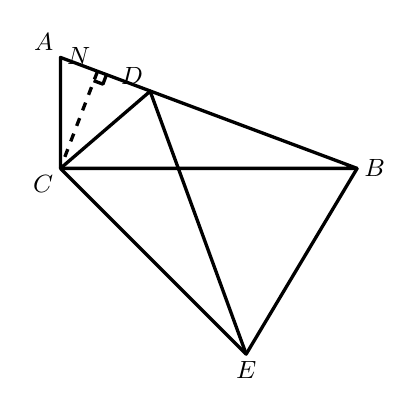
\begin{tikzpicture}[x=0.01cm,y=-0.01cm,line width=1.2pt,line join=round]
% Named points in raw pixel coordinates (y axis flipped via y=-0.01cm)
\coordinate (A) at (54,34);
\coordinate (B) at (431,175);
\coordinate (C) at (54,175);
\coordinate (D) at (168,77);
\coordinate (E) at (290,411);
\coordinate (N) at (101,52);

% Solid edges: AB (through N and D), BC, CA
\draw (A) -- (B) -- (C) -- cycle;
% Solid edges: C-E, E-B, E-D, D-C
\draw (C) -- (E) -- (B);
\draw (E) -- (D) -- (C);

% Dashed perpendicular from C to AB, foot at N
\draw[dashed] (N) -- (C);

% Right-angle mark at N (square of side ~12.6 px, on the C side)
\draw (112.44,56.11) -- (108.0,67.95) -- (96.15,63.52);

% Labels: anchors place text outside each point
\node[anchor=south east,inner sep=2pt] at (A) {\small $A$};
\node[anchor=west,inner sep=2pt] at (B) {\small $B$};
\node[anchor=north east,inner sep=2pt] at (C) {\small $C$};
\node[anchor=south east,inner sep=2pt] at (D) {\small $D$};
\node[anchor=south east,inner sep=2pt] at (N) {\small $N$};
\node[anchor=north,inner sep=2pt] at (E) {\small $E$};
\end{tikzpicture}
\end{document}